%!TEX program = xelatex
% 完整编译: xelatex -> biber/bibtex -> xelatex -> xelatex
\documentclass[lang=cn,a4paper,citestyle=gb7714-2015, bibstyle=gb7714-2015]{elegantpaper}

\title{基于机器学习的煤矿井下瓦斯危害监测预警技术探讨}

\author{姜孟冯\textsuperscript{1,2}}
\institute{(1.中国矿业大学,徐州;\ 2.应急管理部信息研究院,北京)}
\date{\zhtoday}

%%%%%%%%%%%%%%%%%%%%%%%%%%%%%%%%%%%%%%%%%%%%%%%%%%%%%%%%%%%%%%%%%%%%%
% PACKAGES                                                          %
%%%%%%%%%%%%%%%%%%%%%%%%%%%%%%%%%%%%%%%%%%%%%%%%%%%%%%%%%%%%%%%%%%%%%
\usepackage{amssymb}
\usepackage{optidef}
\usepackage{tabularray}
\usepackage{biblatex}
\addbibresource[location=local]{reference.bib} % 参考文献
\usepackage{graphicx}
\usepackage{subcaption}

%%%%%%%%%%%%%%%%%%%%%%%%%%%%%%%%%%%%%%%%%%%%%%%%%%%%%%%%%%%%%%%%%%%%%%
% STYLE ENVIRONMENT                                                %
%%%%%%%%%%%%%%%%%%%%%%%%%%%%%%%%%%%%%%%%%%%%%%%%%%%%%%%%%%%%%%%%%%%%%%
\NewTblrEnviron{research}
\SetTblrOuter[research]{tall}
\SetTblrInner[research]{
    cells  = {c, m},
    hline{1,Z}  = {1pt},% top & bottomrule
    hline{2}    = {0.3pt},% midrule
}
%%%%%%%%%%%%%%%%%%%%%%%%%%%%%%%%%%%%%%%%%%%%%%%%%%%%%%%%%%%%%%%%%%%%%%
% MY COMMANDS                                                        %
%%%%%%%%%%%%%%%%%%%%%%%%%%%%%%%%%%%%%%%%%%%%%%%%%%%%%%%%%%%%%%%%%%%%%%
\newcommand{\R}{\mathbf{R}}
\newcommand{\C}{\mathbf{C}}
\newcommand{\F}{\mathbf{F}}
\newcommand{\U}{\mathit{U}}
\newcommand{\V}{\mathit{V}}
\newcommand{\W}{\mathit{W}}
\newcommand{\poly}{\mathcal{P}}
\newcommand{\espace}{\mathcal{L}}
\newcommand{\expect}{\mathcal{E}}
\newcommand{\mat}{\mathcal{M}}
\newcommand{\mtxA}{\mathcal{A}}
\DeclareMathOperator{\Span}{span}
\DeclareMathOperator{\Real}{Re}
\DeclareMathOperator{\Imag}{Im}
\DeclareMathOperator{\Null}{null}
\DeclareMathOperator{\Range}{range}
\newcommand{\ph}{\phantom{+x_0}}
\newcommand{\mycite}[1]{\textsuperscript{\parencite{#1}}}
\newcommand{\link}[1]{\href{#1}{#1}}


%%%%%%%%%%%%%%%%%%%%%%%%%%%%%%%%%%%%%%%%%%%%%%%%%%%%%%%%%%%%%%%%%%%%%%
% DOCUMENT                                                           %
%%%%%%%%%%%%%%%%%%%%%%%%%%%%%%%%%%%%%%%%%%%%%%%%%%%%%%%%%%%%%%%%%%%%%%
\begin{document}

    \maketitle

    \section{引言}
    井工煤矿作为全球能源开采的关键组成部分,对促进经济发展具有显著影响。尽管如此,矿井环境的复杂性和不确定性显著增加了矿工安全风险,尤其是在瓦斯灾害方面。因此,采用先进的监测预警技术以识别、评估并预测矿井中的瓦斯危害,对于降低事故风险、保障矿工生命安全、减轻经济损失及环境损害具有至关重要的科研价值和实际意义。

    传统的瓦斯危害监测预警方法依赖于物理模型和统计分析,这些方法在处理复杂、非线性和动态变化的环境时存在局限性。随着计算能力的提高和人工智能技术的发展,机器学习(ML)技术因其在处理复杂数据和识别模式方面的优势,被越来越多地应用于瓦斯危害的识别和估计。

    M. Sharma与T. Maity通过研究2000-2022年间瓦斯危害监测领域的论文发表情况,在《Archives of Computational Methods in Engineering》上发表综述性论文\mycite{Sharma2024},探索了基于ML的井工煤矿瓦斯危害识别和监测技术的进展,并比较了传统和基于ML的危害识别方法。

    其论文的主要贡献有:
    \begin{enumerate}
        \item     讨论了流行的预测和估计方法在井工煤矿瓦斯危害识别中的应用。
        \item     对井工煤矿背景下的传统方法与人工神经网络进行了比较。
        \item     解释了现有基于ML的瓦斯危害识别和预测模型的局限性。
    \end{enumerate}

    \section{研究背景和理论基础}
    \subsection{井工煤矿瓦斯危害的研究意义}
    井工煤矿环境具有高度复杂性和挑战性,是潜在危险源的集中区域,其中瓦斯危害是最为显著且严重的威胁之一,尤其在事故原因及死亡统计中占据较大比例。\tabref{tblr:death}展示了有关井工煤矿中各类文献记录的死亡案例数据。由此可见,瓦斯危害在矿井各类灾害中具有较高的普遍性和致命性。因此,针对井工煤矿环境中瓦斯危害的准确识别与风险评估,成为保障矿井安全与减少事故发生的关键研究课题。
    \begin{center}
        \begin{research}[
            caption={常见灾害死亡人数比较},
            entry=none,
            label={tblr:death},
            ]{}
            国家/地区 & 瓦斯爆炸与中毒  & 火灾   & 冲击地压与顶板   & 水灾   & 其他 \\
            中国, 2001–2015\mycite{Meng2019} & 64.72 & 4.08 & 8.46 & 16.84 & 5.9\\
            印度, 2001–2014\mycite{Tripathy2018} & 3.36 & – & 55.14 & – & 41.5\\
            波兰, 2008–2017\mycite{ref14} & 82.2 & 0.0 & 15.6 & 2.2 &0.0\\
            美国, 1900–2006\mycite{Kowalski-Trakofler2009} & 89.52 &6.26 &0.71&–&3.51\\
        \end{research}
    \end{center}

    \subsection{瓦斯监测系统的研究}
    井工煤矿瓦斯监测系统的研究和开发历史悠久,其目标是实现井下各类环境参数的实时监测与危险报警,以保障矿井生产安全。多数煤矿实际使用的瓦斯监测系统,对各类重要传感器设有报警门限阈值,一旦监测值超过报警阈值,则及时通知煤矿调度管理人员,及时对正在报警的灾害问题进行处置。而关于煤矿瓦斯危害预测预警方面的研究,仍处于产学研讨阶段,未进入实际工业大规模使用。

    传统的监测方法依赖于物理模型和统计工具,如线性回归,来分析气体浓度模式。然而,这些方法通常只能处理单一属性,而气体浓度可能受到环境和通风状态等多种因素的影响。此外,井工煤矿中的气体浓度表现出非线性和复杂的关系,难以通过物理模型实现。

    \subsection{机器学习在瓦斯监测预警中的应用}
    近些年来,一些人工智能(AI)方法被应用在了瓦斯危害监测预警领域,基于人工智能的深度神经网络(DNN)模型可以提取各种属性之间的非线性复杂规则,从而得出专门的解决方案。研究\mycite{Tutak2019a}提出了基于人工神经网络(ANN)的甲烷预测模型。该研究针对煤矿井下的不同位置提出了多个多层感知(MLP),所有 MLP 都取得了显著的预测结果。除甲烷相关研究外,Bonetti 等人\mycite{Bonetti2019}等人的几项研究也提出了对包括甲烷在内的其他气体的监测。

    气体监测和估算是瓦斯监测系统的一个方面,另一个方面是传感器节点之间的通信--瓦斯危害监测系统强依赖于传感器节点之间的可靠通信。有线通信系统是井工煤矿的传统方法。然而,动态和复杂的工作环境带来了各种严峻的挑战,如有线通信装置的机械损坏。因此,Chen 和 Wang \mycite{Chen2020} 以及 Muduli 等人\mycite{Muduli2018b}等人的多项研究都旨在利用无线网络的优势开发无线传感器网络 (WSN)。然而,地下矿井的几何形状和煤炭特性限制了 WSN 的全面实施。这些网络问题也会对瓦斯监测预警带来限制,后文会详细讨论。

    \section{传统的瓦斯危害预测评估方法}
    \subsection{卡尔曼滤波}
    卡尔曼滤波(Kalman Filtering)是一种高效率的递归滤波器(自回归滤波器),它能够从一系列的不完全及包含噪声的测量中,估计动态系统的状态。卡尔曼滤波会根据各测量在不同时间下的值,考虑各时间下的联合分布,再产生对未知变量的估计,因此会比只以单一测量量为基础的估计方式要准。


    \subparagraph*{卡尔曼滤波器的状态:} 由以下两个变量表示:

    \begin{itemize}
        \item     ${\hat{\textbf{x}}}_{k|k}$,在时刻k的状态的估计;
        \item     ${\textbf{P}}_{k|k}$,后验估计误差协方差矩阵,度量估计值的精确程度。
    \end{itemize}

    \subparagraph*{卡尔曼滤波器的操作:} 包括两个阶段:\textbf{预测}与\textbf{更新}。

    \subparagraph*{(1)预测的过程:}使用上一状态的估计,做出对当前状态的估计。
    \begin{itemize}
        \item   预测状态,如(\ref{eqn:kalman1})所示:
        \begin{equation}
            {\hat {\textbf {x}}}_{k|k-1}={\textbf {F}}_{k}{\hat {\textbf {x}}}_{k-1|k-1}+{\textbf {B}}_{k}{\textbf {u}}_{k}
            \label{eqn:kalman1}
        \end{equation}
        \item   预测估计协方差矩阵,如(\ref{eqn:kalman2})所示:
        \begin{equation}
            {\textbf {P}}_{k|k-1}={\textbf {F}}_{k}{\textbf {P}}_{k-1|k-1}{\textbf {F}}_{k}^{T}+{\textbf {Q}}_{k}
            \label{eqn:kalman2}
        \end{equation}
    \end{itemize}

    \subparagraph*{(2)更新的过程:}利用对当前状态的观测值优化在预测阶段获得的预测值,以获得一个更精确的新估计值。
    \begin{enumerate}[label=\alph*.]
        \item 首先计算三个变量:\begin{itemize}
            \item   测量误差,如(\ref{eqn:kalman3})所示:
            \begin{equation}{\tilde {\textbf {y}}}_{k}={\textbf {z}}_{k}-{\textbf {H}}_{k}{\hat {\textbf {x}}}_{k|k-1}
                \label{eqn:kalman3}
            \end{equation}
            \item   测量误差协方差,如(\ref{eqn:kalman4})所示:
            \begin{equation}{\textbf {S}}_{k}={\textbf {H}}_{k}{\textbf {P}}_{k|k-1}{\textbf {H}}_{k}^{T}+{\textbf {R}}_{k}
                \label{eqn:kalman4}
            \end{equation}
            \item   最优卡尔曼增益,如(\ref{eqn:kalman5})所示:
            \begin{equation}{\textbf {K}}_{k}={\textbf {P}}_{k|k-1}{\textbf {H}}_{k}^{T}{\textbf {S}}_{k}^{-1}
                \label{eqn:kalman5}
            \end{equation}
        \end{itemize}
        \item 然后用它们来更新滤波器状态: \begin{itemize}
            \item  更新状态估计,如(\ref{eqn:kalman6})所示:
            \begin{equation}{\hat {\textbf {x}}}_{k|k}={\hat {\textbf {x}}}_{k|k-1}+{\textbf {K}}_{k}{\tilde {\textbf {y}}}_{k}
                \label{eqn:kalman6}
            \end{equation}
            \item  更新协方差估计,如(\ref{eqn:kalman7})所示:
            \begin{equation}{\textbf {P}}_{k|k}=(I-{\textbf {K}}_{k}{\textbf {H}}_{k}){\textbf {P}}_{k|k-1}
                \label{eqn:kalman7}
            \end{equation}
        \end{itemize}
    \end{enumerate}

    \bigskip
    只有极少数文献专门介绍了卡尔曼滤波在井工煤矿瓦斯危害预测中的应用。文献\mycite{Wu2018} 采用了集合卡尔曼滤波器来估算主回风道中的甲烷扩散。该模型的开发考虑了回气道的静态和规则结构。但井工煤矿环境是动态的,而且非常复杂,因此用数学方法来解释具有挑战性。因此,设计物理模型和测量模型成为一项具有挑战性的任务。这项技术的另一个问题是其可扩展性。也就是说,随着矿山几何形状的变化,需要重新设计物理模型和测量模型。
    \subsection{最小二乘法}
    最小二乘法(Least Square)又称最小平方法,是一种数学优化建模方法。它通过最小化时间序列上的预测误差的平方和寻找数据的最佳函数匹配,如(\ref{eqn:lstsqr})所示:
    \begin{equation}
        min \sum_{i=1}^{n}(y - H\cdot \hat{x})^2
        \label{eqn:lstsqr}
    \end{equation}
    (\ref{eqn:lstsqr})中,$y$ 是任何过程的输出,$\hat{x}$是估计状态,$H$ 是测量矩阵。通过求解优化问题,可以找到最佳估计状态。

    \bigskip
    最小二乘法的其他变种是加权最小二乘法和递归最小二乘法。这是一种通过最小化数据点与回归线之间的平方距离来估计参数的方法。对于井工煤矿案例,文献\mycite{ref81} 使用这种方法来估计线性回归模型的参数,以预测甲烷浓度。这种方法的缺点是需要在程序之前建立回归模型。在许多情况下,可能需要使用多个回归模型进行测试,以获得最佳模型,这不仅耗费时间,还会导致估算结果仅仅是次优解。

    \subsection{最大似然法}
    最大似然法(Maximum Likelihood)是另一种参数估计技术;与最小二乘法不同,该模型考虑了观测样本的概率分布函数(PDF)。似然函数可表示为(\ref{eqn:maxlike}):
    \begin{equation}
        L(W|Y) = f(y_1|W)f(y_2|W)f(y_3|W)\cdots f(y_k|W)
        \label{eqn:maxlike}
    \end{equation}
    (\ref{eqn:maxlike})中,$f$表示 PDF,$W$是参数向量,$Y$是样本向量,$y_1 - y_k$ 是样本向量$Y$的元素。

    要获得$W$参数的最大似然估计(MLE),可令似然函数$L$关于$W$向量中所有参数的一阶偏导数为0,如(\ref{eqn:maxlikegrad})所示:
    \begin{equation}
        \dfrac{\partial L(W|Y)}{\partial w_i}=0
        \label{eqn:maxlikegrad}
    \end{equation}
    $w_i$是 $W$ 的第 $i$个元素,利用(\ref{eqn:maxlikegrad}),可以得到与 $W$ 相关的估计参数。关于 MLE 的更多详情,请参见文献\mycite{Myung2002}。

    在井工煤矿案例中,文献\mycite{Asfaw2013} 使用 MLE 对负二叉模型中的伤害变量指标模型进行参数估计。除这项工作外,在使用 MLE 进行井工煤矿瓦斯危害预测领域还没有重要研究。同样,该方法考虑了已知 PDF 模型及其待估算参数。然而,就井工煤矿而言,由于可用数据有限,且不同矿井之间存在差异,因此使用 MLE 设计通用危害预测模型具有挑战性。

    \subsection{基于知识的专家系统}
    基于知识专家系统(KBES)主要依赖传感器数据作为输入,这些数据可能包括图像、温度、湿度等环境参数,或者是任何其他可以通过传感器监测到的信息。KBES通过分析输入数据与知识库中的相关性来制定决策。知识库由一系列简单的语法规则和决策参数模板构成,通常采用“如果-那么”(IF-Then)语句的形式。关于这种方法的详细信息,可以参考文献\mycite{ref59}。

    \bigskip
    相比之下,这种模型属于较为简单的技术类别,能够直接应用于微控制器等小型传感器设备上。因此,大多数用于煤矿气体检测的传感器都采用了这种方法。文献\mycite{Reddy2021}介绍了一种基于物联网的矿井安全系统,该系统利用Arduino控制器、瓦斯传感器接口和扬声器作为报警指示器。当瓦斯浓度超过最大允许值时,扬声器会发出警报。文献\mycite{Singh2022}提出了一种用于监测煤矿环境的物联网智能头盔,该头盔通过传感器收集数据,并利用微控制器将数据传输至云服务器。在云服务器中,传感器数据与一系列预定义的规则进行匹配,以生成报警信号。文献\mycite{Sarkar2021}提出了一种矿井危险报警系统,旨在减轻火灾、水患和地层风险。该系统整合了与这些模式相关的微控制器传感器,并使用专门的规则库来识别危险。文献\mycite{ref25}\mycite{Huang2015}\mycite{Nie2014}中也报道了类似的研究,它们都采用了专门的危险识别知识库。

    \subsection{模糊集理论}
    基于模糊集理论(Fuzzy Set Theory)的推理模型适用于输入数据模糊或输入数据被模糊化的情况\mycite{Khaleghi2013}。对于主要由语言变量表示的模糊数据,它包括两个步骤。第一步是为推理模型建立一个模糊规则库,如(\ref{eqn:fuzzysetrule})所述。
    \begin{equation}
        \begin{aligned}
            R : \\
            &IF(A_1\ is\ S_{i1}\ AND\ A_{2}\ is\ S_{i2}\ AND\ A_3\ is\ S_{i3} \dots AND\ A_k\ is\ S_{ik})\\
            &THEN (O\ is\ D)
        \end{aligned}
        \label{eqn:fuzzysetrule}
    \end{equation}

    上述模糊规则具有 “IF-THEN ”结构,包含一些语句。与 “IF ”相关的语句是前件,与 “THEN ”相关的语句是后件。前件是各种属性($A_1 - A_k$)与其第 $i$ 个语言变量($S_1 - S_n$)的组合,使用 AND、OR 和 NOT 等逻辑运算符。此外,与 “THEN ”相关的结果语句是用语言变量 D 表示的输出 O。整个过程就是将模糊输入变量应用到模糊推理模型中,利用预定义的规则集进行推理,得出模糊输出,再利用去模糊化过程将其转换为确定值。

    模糊集理论的另一种情况是,输入是一个确定的数字,但通过模糊化过程转换为模糊变量。在这一过程中,如(\ref{eqn:fuzzyset})所述,每个确定输入变量都使用成员函数与语言变量相关联。
    \begin{equation}
        F =  \{(x, \mu_k(x)) : \forall x \in X\}
        \label{eqn:fuzzyset}
    \end{equation}
    在(\ref{eqn:fuzzyset})中,$F$ 表示确定输入 $x$ 的模糊变量集,$\mu_k$ 表示在 [0,1] 范围内第 $k$ 个模糊变量的成员函数。关于这种方法的更多细节,可参考文献\mycite{Muduli2018a}。

    \bigskip
    由于这种方法不依赖于任何物理模型或历史数据,它在井工煤矿中得到了广泛应用,特别是在火灾和瓦斯相关的危害控制方面。文献\mycite{Li2020}探讨了基于模糊层次分析法(AHP)的贝叶斯网络在爆炸危险性评估中的应用。研究中考虑了多种因素,包括通风故障、密封质量、人为错误和仪器误差,并通过对多个领域的专家进行问卷调查,收集了基于模糊AHP的这些因素发生概率的数据。文献\mycite{Danish2020}则介绍了对井工煤矿火灾强度的研究,其中O2、N2、CO和温度的浓度作为模糊推理系统的输入。所有输入数据都通过梯形隶属函数进行模糊化处理,而模型的模糊输出则通过区域中心点(COA)方法进行去模糊化处理。文献\mycite{Mahdevari2014}提出了一种基于模糊TOPOSIS的危害缓解方法,该方法综合考虑了井工煤矿中的多种危害因素,包括地质学、电气、机械、化学、环境、个人和社会因素,并利用模糊TOPOSIS对这些因素进行排序。文献\mycite{Basu2019}也探讨了基于各种气体的井工煤矿火灾强度监测,但采用的是2型模糊逻辑控制器。2型控制器的优势在于能够模拟1型模糊控制器成员函数中的不确定性。类似的。文献\mycite{Brodny2022}和Shi等人\mycite{Shi2018}介绍了基于模糊逻辑的井工煤矿危害监测系统的另一版本。


    \subsection{贝叶斯网络}
    贝叶斯网络(Bayesian Network, BN)又称信念网络(Belief Network)或是有向无环图模型(Directed Acyclic Graphical Model),是一种概率图型模型,通过有向无环图(DAG)表示一组随机变量$\left\{X_{1},X_{2},...,X_{n}\right\}$及其条件概率分布(Conditional Probability Distributions, CPD)的性质。

    令$G = (I,E)$ 表示一个有向无环图(DAG),其中 $I$ 代表图中所有的节点的集合,而 $E$ 代表有向连接线段的集合,且令 $X = (X_i)i\in I$为其有向无环图中的某一节点 $i$ 所代表之随机变量,若节点 $X$ 的联合概率分布可以表示成(\ref{eqn:bn}):
    \begin{equation}
        p(x)=\prod _{i\in I}p{\big (}x_{i}\,{\big |}\,x_{\operatorname {pa} (i)}{\big )}
        \label{eqn:bn}
    \end{equation}
    则称 $X$ 为相对于有向无环图 $G$ 的贝叶斯网络,其中
    $pa(i)$表示节点 $i$ 之“因”。(即通过单边直接指向i的顶点)

    一般而言,贝叶斯网络的有向无环图中的节点表示随机变量,它们可以是可观察到的变量,抑或是隐变量、未知参数等。箭头表示因果关系或条件独立性,无箭头表示条件独立性,单箭头连接表示因果关系,两个节点就会产生一个条件概率值。大部分情况下,贝叶斯网络适用在节点的性质是离散型的,可依照
    $ P(X_{i}|P_{i})$此条件概率写出条件概率表,此条件概率表的每一行列出所有可能发生的
    $P_{i}$,每一列列出所有可能发生的$X_{i}$,且全部行的概率总和必为1。有关这方面的更多详细信息,可以参见 Stephenson\mycite{Stephenson2000}。

    \bigskip
    贝叶斯网络在井工煤矿危害缓解中的应用已经得到了广泛的研究。文献\mycite{Tong2018}显示,将贝叶斯网络与德尔菲法结合使用,是评估矿井爆炸危险的有效工具。Zhang等人提出了一种基于加权贝叶斯网络的瓦斯突出预测模型\mycite{Zhang2021}。在不同指标下的后验概率会根据指标间的熵值进行加权。然后,使用加权后的后验概率来计算瓦斯突出的概率。在文献\mycite{Li2019}中,Li等人研究了用于矿井点火源风险评估的模糊贝叶斯网络。他们采用了模糊层次分析法(AHP)模型,以整合不同领域专家基于他们的专长、知识、教育水平和其他参数的决策。类似的研究也可以在文献\mycite{ref23}\mycite{ref34}\mycite{ref47}\mycite{ref48}中找到。
    \section{基于机器学习/人工神经网络的瓦斯危害预测与评估方法}
    人工神经网络(Artificial Neural Network,ANN)是受生物学启发的数学模型,由称为神经元的处理元件组成。每个神经元通过一个称为权重的系数连接起来\mycite{Shanmuganathan2016}。\figref{fig:ann-architecture-1} 描述了 ANN 的基本结构。与前面讨论的模型不同,ANN 不需要明确的建模来完成检测或分类任务。因此,对于数学建模不可能或资源效率不高的复杂物理现象,ANN 是一个合适的候选模型。这些基于监督学习的数据驱动模型在基本操作和架构上各不相同。在井工煤矿瓦斯危害案例中,人工神经网络被广泛用于预测和预警目的。这些模型大致可分为两类,浅层神经网络和深层神经网络(DNN)。
    \begin{figure}[!h]
        \centering
        \begin{subfigure}[b]{0.4\textwidth}
            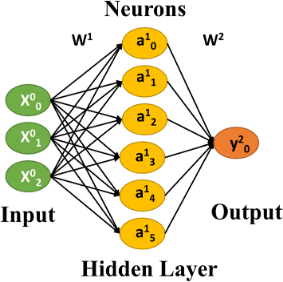
\includegraphics[width=\textwidth]{ann-architecture-1}
            \caption{ANN计算结构}
            \label{fig:ann-architecture-1}
        \end{subfigure}
        \hfill
        \begin{subfigure}[b]{0.5\textwidth}
            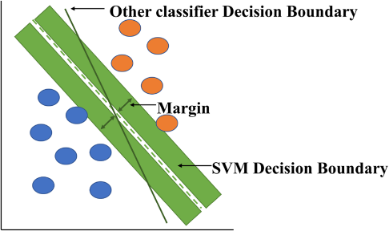
\includegraphics[width=\textwidth]{ann-architecture-2}
            \caption{ANN对比SVM}
            \label{fig:ann-architecture-2}
        \end{subfigure}
        \caption{ANN结构图}
    \end{figure}
    \subsection{浅层神经网络模型}
    浅层神经网络(Shallow Neural Network)是一类特殊的神经网络模型,其隐藏层数相对少于 DNN。与 DNN(如卷积神经网络(CNN)或循环神经网络(RNN))相比,这些模型的复杂性较低。支持向量机和具有单个隐藏层的 ANN 是这类模型中的常用模型。浅层神经网络的基本结构如\figref{fig:ann-architecture-1}所示,相关计算过程大都分为两个步骤,即前向传播和后向传播。下面将简要讨论这两个过程。

    \subparagraph*{前向传播:}输入向量与权向量的内积后,经一个非线性传递函数得到一个标量结果输出。\figref{fig:ann-architecture-1}中网络的前向传播的典型方式以公式(\ref{eqn:ann-fp})中给出。
    \begin{equation}
        A^1 = g\{\{W^1\}^T \cdot X+B^1\}
        \label{eqn:ann-fp}
    \end{equation}
    其中$A^1$是隐藏层“1”的激活,$W^1$是与隐藏层“1”和前一层相关的权重矩阵,$X$是前一层的向量形式输入,$B^1$是与层“1”相关的偏置。在(16)中,$g$代表非线性激活函数,如sigmoid、tanh 和 RELU。

    \subparagraph*{后向传播:}根据梯度下降算法更新每一层的权重或系数。先利用损失函数计算实际值与估计值之间的差,再计算损失函数的梯度,并将其反向传播至整个网络。损失函数可表示如(\ref{eqn:ann-bp1})所示,
    \begin{equation}
        J= \dfrac{1}{2m} \sum_{i=0}^{m} (y_i - \hat{y_i})^2
        \label{eqn:ann-bp1}
    \end{equation}
    J 为损失函数。如此,就可以用梯度下降算法更新不同层的参数$W$\mycite{ref77},表示如(\ref{eqn:ann-bp2})所示:
    \begin{equation}
        W = W - \alpha\frac{\delta J}{\delta W}
        \label{eqn:ann-bp2}
    \end{equation}
    其中 $\alpha$ 是称为学习率的超参数,$\frac{\delta J}{\delta W}$ 是损失函数相对于参数 W 的梯度。

    \subparagraph*{支持向量机(Support Vector Machine, SVM):}相比之下,支持向量机(SVM)这种大边界分类器在决策边界方面与传统的人工神经网络(ANN)模型有所不同。SVM在决策边界周围实现了额外的边界,如\figref{fig:ann-architecture-2}所示,这在基于ANN的模型中是不常见的\mycite{Moraes2013}。因此,与基于ANN的分类器相比,SVM能提供更准确的决策。

    \bigskip
    这些模型均可用于井工煤矿场景中的瓦斯浓度预测。文献\mycite{Xiao2011}介绍了一种用于减轻井工煤矿自燃煤危险程度的反向传播ANN(BP-ANN)模型,并利用遗传算法对模型参数与训练性能进行了优化。文献\mycite{Xu2020}介绍了一种基于无痕卡尔曼滤波器(UKF)的BP-ANN模型,声称UKF可用来调整BP-ANN模型参数,使系统对故障具有鲁棒性,并具有较高的决策精度,但并未验证有效性。文献\mycite{Tutak2019b}提出了一个多层感知器模型,用于预测井工煤矿的甲烷浓度,并研究了不同结构对预测未来15分钟内甲烷浓度的影响。文献\mycite{Barros-Daza2022}提出了一个ANN模型,使用井工煤矿的可测量参数(如CO、CO2、O2、空气流速等)来分类火灾危害等级。研究表明,该模型的分类准确率达到了97\%。类似的研究\mycite{He2010}\mycite{Jo2018}\mycite{Ruilin2010}\mycite{Xie2019}建议将ANN作为井工煤矿场景中瓦斯危害预测的可靠模型。

    与涉及ANN的研究相对照,大量的文献也涉及了基于SVM的模型。文章\mycite{Deng2018}提出了一个与粒子群优化(PSO)集成的基于SVM的回归模型。该模型旨在使用当前气体(如CO和CO2)预测采空区内的煤炭自燃温度。与BP-ANN模型相比,基于SVM的回归模型在温度预测上更为准确。文献\mycite{Lei2019}对随机森林(RF)模型和支持向量机(SVM)在预测井工煤矿煤炭自燃温度方面的应用进行了系统的对比分析。通过主成分分析(PCA)技术,研究者们生成了一组降维后的特征集。分析发现,SVM的性能在很大程度上受到超参数选择的影响。相比之下,随机森林模型显示出对SVM的优越性,具有更强的鲁棒性和更高的预测准确度。尽管如此,正确选择SVM的超参数也能显著提高其预测性能。

    文献\mycite{Tripathy2021}中的一项研究系统评估了K最近邻(KNN)、逻辑回归(LR)、决策树(DT)和支持向量机(SVM)在矿井危害分类中的效能。研究筛选了17个关键输入变量,涵盖井工矿安全的关键领域,并计算了这些变量的均值、方差、四分位数和最大值等统计属性。结果表明,除DT外,其余模型在准确度和F1分数上均呈现可接受的分类性能。在支持向量机的变体中,最小二乘-支持向量机(LSSVM)亦被纳入井工煤矿瓦斯危害的讨论。文献\mycite{Cao2008}利用LSSVM分析了甲烷相关的瓦斯危害,并构建了一个预测与预警模型,声称具有高精度和可靠的预警能力,但未与其他方法进行比较验证。其他基于LSSVM对井工煤矿危害进行研究的工作见于文献\mycite{Chou2016}\mycite{Yang2013}\mycite{Zhao2009}。

    \subsection{深层神经网络(DNN)模型}
    深层神经网络(Deep Neural Network, DNN)与 ANN 和 SVM 等浅层神经网络不同,DNN 架构由2层以上的隐藏层组成,通常具有复杂的神经网络,也称为深度 ANN(DANN)。卷积神经网络(CNN)和循环神经网络(RNN)是研究最多的基本 DNN 模型。DNN 的运行基本原理与 ANN 相同,只是它的网络结构更大、更复杂。下文将讨论 CNN 和 RNN 的基本原理。

    \begin{figure}[!h]
        \centering
        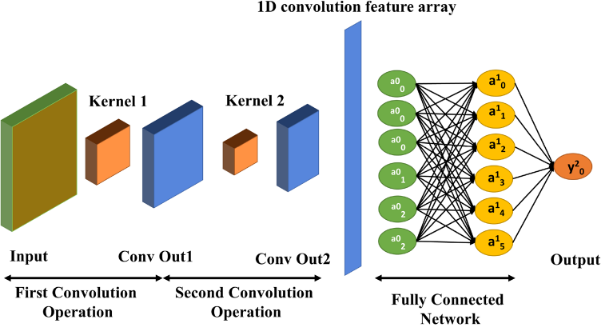
\includegraphics[width=0.5\textwidth]{cnn-based-model}
        \caption{CNN基本模型}
        \label{fig:cnn-based-model}
    \end{figure}

    \subsubsection{卷积神经网络(CNN)模型}
    卷积神经网络(Convolution Neural Network, CNN),这些模型通常用于空间特征提取。与其他需要手动提取特征的 DNN 模型相比,CNN 模型的自动特征提取能力具有额外的优势\mycite{Alzubaidi2021}。CNN 架构的基本结构如\figref{fig:cnn-based-model}所示。与 ANN 架构不同,CNN 在输入和内核之间执行卷积运算。输入块是一个形状为 $(h \times w \times c)$ 的张量,其中 “$h$”表示行数,“$w$”表示列数,“$c$”表示通道数。内核块类似于 ANN 架构中的神经元,包含可以在输入中卷积的特定权重。内核块也是一个张量,其形状为$(a \times b \times c)$,其中 “$a$”为内核的高度,“$b$”为内核的宽度,“$c$”为通道数。值得一提的是,内核和输入的通道数应相同。“卷积输出”(Conv out)模块表示存储从卷积过程中提取的特征的张量。关于这一上下文的更多细节,可以参考文献\mycite{ref29}。
    \bigskip
    尽管基于 ML 的 井工煤矿情景模型还处于研究的初始阶段,但基于 CNN 的瓦斯突出预测模型已经问世。文献\mycite{Li2021}利用声发射(AE)和电磁辐射(EMR)信号,提出了基于 CNN 的煤岩爆发危险。AE 和 EMR 信号最初使用经验模式分解(EMD)进行修改,然后转换成二维张量供 CNN 输入。作者使用了一种间接方法来预测岩石和瓦斯爆发,即使用 EM 和 EMR 而不是瓦斯浓度。文献\mycite{Zhang2018} 提出了基于 RFID 的甲烷浓度预测模型。预测算法基于集成的 CNN-LSSVM 算法。CNN 用于从使用 RFID 标签的行传感器数据中提取稳健特征,并使用 LSSVM 模型进行预测。文献\mycite{Qiu2022} 的作者使用 K-NN 与 CNN 集成建立了瓦斯危害分类和预测模型。K-NN 用于对异常瓦斯浓度源进行分类,CNN 用于预测爆破过程导致的爆发风险。
    \begin{figure}[!h]
        \centering
        \begin{subfigure}[b]{0.5\textwidth}
            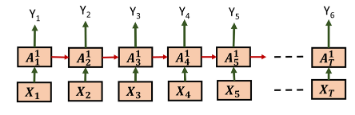
\includegraphics[width=\textwidth]{rnn-architecture}
            \caption{RNN层状结构}
            \label{fig:rnn-architecture}
        \end{subfigure}
        \begin{subfigure}[b]{0.4\textwidth}
            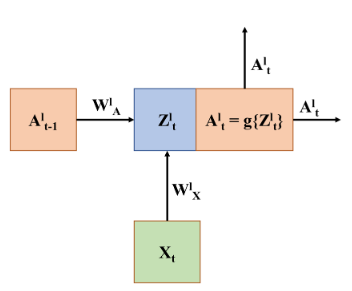
\includegraphics[width=\textwidth]{rnn-cell}
            \caption{RNN单元}
            \label{fig:rnn-cell}
        \end{subfigure}
        \caption{RNN结构图}
    \end{figure}

    \subsubsection{循环神经网络(RNN)模型}
    循环神经网络(Recurrent Neural Network, RNN),RNN 在结构上与 ANN 相似,但多了一些时序结构。
    这种时序结构可提取任何时间序列中的时序特征。RNN 的基本结构如\figref{fig:rnn-architecture}所示。在 RNN 结构中,$X_1-X_T$ 表示时序数据列,$A_1^1-A_1^T$是给定时间戳 $1-T$ 的提取特征。上述符号中的下标表示时间戳,上标表示层数。此外,RNN 架构中一个时间戳操作的直观框图如\figref{fig:rnn-cell} 所示。\figref{fig:rnn-cell} 所示的RNN 单元有两个输入,一个来自相应时间戳的实际输入($X_t$),另一个来自上一个时间戳($A^l_{t-1}$)。RNN 的其他变体包括门控递归单元(GRU)和长短期记忆(LSTM)。普通 RNN、LSTM 和 GRU 之间的基本区别在于,它们都有通过某种门控机制运行的记忆保持单元。这种记忆单元有助于在较长的时间样本中保持时间特征。有关 RNN 模型及其变体的详细信息,可参见文献\mycite{ref79}。

    \bigskip
    基于 RNN 的模型在煤矿甲烷浓度预测中的应用在最近的文献中很明显。文献\mycite{Xu2022} 介绍了井工煤矿中基于 LSTM 的门烷烃气体浓度预测。文献使用鲸鱼优化算法(Whale Optimization Algorithm, WOA)对 LSTM 的超参数进行了优化,并引入了输入序列的经验模态分解(Empirical Mode Decomposition, EMD)方法以获取各个内在模态函数(Intrinsic Mode Function, IMF)作为LSTM的输入。在文献\mycite{Kumari2021}中,研究者提出了一种基于均匀流形近似和投影(Uniform Manifold Approximation and Projection, UMAP)和LSTM的矿井火灾预测模型,该模型利用了多种属性气体,如O2、CO、CO2、CH4、H2、N2和C2H4。与传统的机器学习方法(如支持向量机SVM和自回归积分滑动平均模型ARIMA)相比,所提出的模型在效率上有显著提升。文献\mycite{Meng2022}和Dey等人\mycite{Dey2021b}也利用基于LSTM的模型对煤矿中的瓦斯危害进行预测。

    \subsubsection{其他模型}
    除 CNN 和 RNN 模型外,一些文献,如 Dey 等人\mycite{Dey2021a}和 Hati 等人\mycite{Hati2022},主张使用混合 CNN-LSTM 模型进行煤矿瓦斯浓度预测。混合架构利用了两者的优点,即从 CNN 自动提取特征并保持提取特征之间的时间完整性。与独立的 CNN 或 RNN 模型相比,这些混合模型表现出更好的性能。

    \section{传统与机器学习模型的比较}
    本节将在井工煤矿场景下对上述算法进行比较。 这有助于筛选出最适合井工煤矿场景的传感器融合算法。比较结果见\tabref{tblr:models}。

    \begin{center}
        \begin{research}[
            caption={井工煤矿瓦斯监测预警模型比较},
            entry=none,
            label={tblr:models},
            ]{
                column{1} = {c,wd=.15\linewidth},
                column{2} = {l,wd=.4\linewidth},
                column{3} = {l,wd=.45\linewidth},
                row{1} ={c}
            }
            模型 & 优势  & 劣势 \\
            卡尔曼滤波 & {1.与数据驱动模型相比更精确\\2.卡尔曼滤波有效地考虑了过程模型和测量模型噪声} & {1.卡尔曼滤波只适用于定义明确的物理模型\\2.非线性过程模型的实现非常复杂,而且计算成本高昂} \\
            最小二乘法 & {1.建模简单\\2.不需要先前的信息\\3.不需要物理模型} & {1. 需要预定义模型,不适合动态复杂的过程\\2.无法灵活应对输入参数的数量变化} \\
            最大似然法 & {1.使用概率分布函数PDF而不是曲线拟合可以提高估计精度\\2.不需要物理模型} & {1. 需要事先了解与正在研究的参数相关的概率分布函数PDF\\2.小样本的估计值可能会有偏差\\3.模型的复杂度取决于似然函数的选择} \\
            贝叶斯网络 & {1.不需要物理模型\\2.适用于小数据样本\\3.可结合不同的知识来源} & {1. 需要事先计算先验概率分布\\2.对于多个假设和多个条件依赖项计算复杂\\3.需要适用于贝叶斯网络模型的条件概率表\\4.一次只考虑两个假设} \\
            基于知识的专家系统 & {1.设计简单\\2.不需要物理模型} & {1.需要预定义的规则库\\2.无法处理测量中的不确定性\\3.当出现轻微的测量偏差时,可能会导致错误的决策} \\
            模糊集理论 & {1.可以有效处理数据样本中的模糊性\\2.\ 2型模糊推理模型可处理数据不确定性\\3.不需要物理模型} & {1.需要预定义的规则库\\2.仅支持识别或分类任务,不适合预测} \\
            神经网络 & {1.不需要精确的物理模型\\2.仅使用历史数据了解与流程相关的规则\\3.不需要概率分布的先验知识} & {1.特征工程步骤可能很耗时\\2.是黑盒模型\\3.与其他模型相比,计算很复杂} \\
        \end{research}
    \end{center}

    考虑到井工煤矿场景中动态且复杂的环境,建立瓦斯危害监测过程的物理模型难以实现。即使是文献中的研究,如 Wu 等人\mycite{Wu2018},也是基于带有若干假设的近似物理模型。目前尚未有关于使用物理模型进行瓦斯危害预测和缓解的实际应用报告。因此,物理模型并不适合瓦斯危害预测任务。由于瓦斯浓度及其危害之间的非线性关系,基于最大似然法和最小二乘法的模型也不适合相关目的。因此,关于卡尔曼滤波、最小二乘或最大似然的文献非常有限。

    与\tabref{tblr:models}中的前几种模型相比,贝叶斯模型不像最小二乘法或最大似然法那样受任何预定义数学模型的约束,而是需要条件概率表,但这却需要按照多重假设与条件依赖事件进行繁琐地设计,实质上也难以实现。更糟的是,所有这些模型都严重受到数据不确定性和模糊性的影响。恶劣和动态的井下环境使得基于传感器的监测容易受到各种噪声测量的影响,从而给数据带来不确定性。

    模糊集理论和基于Dempster-Shafer证据理论的模型能够处理数据中的不确定性和模糊性。因为推理引擎是在人类专家和认知智能的帮助下开发的,这些模型在信息量非常小的情况下非常有用。然而,这些模型不适用于模式识别或预测任务。

    与其他传感器融合算法不同,人工神经网络(ANN)和深度神经网络(DNN)能够发现任何过程输入和输出变量之间的非线性关系。事实证明,这些模型对于高度复杂的非线性过程非常有效。此外,像ANN或SVM这样的浅层神经网络容易受到噪声数据的影响,但像卷积神经网络(CNN)这样的DNN模型能够处理噪声数据。神经网络高效的模式识别能力使它们成为井工煤矿危害识别模型的合适选择。然而,当传感器出现任何故障时,就会发现这些数据驱动模型存在很大的局限性。故障传感器可能会导致错误的观测结果,从而导致错误的估计或预测。目前还没有文献涉及这一实际问题,大多数研究主要关注于设计通用的数据驱动模型。

    \section{神经网络模型的挑战和局限性}
    表 5 中讨论的模型访问煤矿井下的传感器数据,以处理推断操作。完整的推理过程包括数据收集、数据工程、模型准备和模型部署。在数据工程步骤中,从行列传感器数据中提取特征并规范化,以用于训练和验证。然而,这种方法存在以下局限性:

    1. 在井工煤矿危害监测中实施 DNN 的文章数量很少。

    2. 所有危害预测模型都采用了单模型方法,即单个网络专用于在进行预测时,需要考虑单个参数。然而,该参数的预测可能会受到其他因素的影响,而这些因素在目前的文献中都没有考虑到。

    3. 实际传感器数据通常因各种因素而具有不确定性。例如,甲烷传感器的读数为 12,000 ppm,阈值为 12,500 ppm,而测量不确定性为 5\%,则可能无法确定传感器观测值是低于阈值还是高于阈值。

    4. 所有神经网络模型都是根据确定的传感器值进行训练的,没有考虑传感器的不确定性,这可能会降低实时情况下的准确性。

    5. 如果传感器发生故障,问题可能会持续存在。由于地下环境恶劣且复杂,传感器故障在井工煤矿中频繁发生且不可避免。在井工煤矿危害监测研究中已观察到故障节点情况的证据。文献\mycite{Schatzel2017}中的研究发现,在煤矿实验的第三天,某个甲烷传感器出现故障。与其他甲烷监测器相比,甲烷浓度偏高。另一项文献研究\mycite{Krog2006}也报告了类似事件。传感器观测到的故障可能会导致超出分布范围(OOD)的情况,可以使用一些统计异常检测方法轻松处理。但是,故障并不总是能超出分布范围,如果发生这种情况,估计或分类过程的准确性就会大大降低。

    6. 动态和复杂的井工煤矿环境对传统的危害监控系统造成了许多限制。根据对各种文献的调查,与煤矿传感器网络相关的重大挑战如下。 (a) 在一个矿井巷道完成煤炭开采后,需要将整个机械和基础设施转移到下一个作业区。这一拆卸和重新安装过程对传统的有线通信基础设施造成了限制。(b) 此外,有线通信网络容易受到机械和其他方面的损坏。(c) 在这种情况下,无线基础设施在灵活性和便携性方面具有优势。然而,井工煤矿的地下作业对传统无线系统造成了限制。 (d) 此外,由于煤的介电性能和井工煤矿的地质特征,这些无线系统的信号衰减很大。

    \section{可能的解决方案}
    使用基于 Dempster-Shafer 证据理论(DSET)的多标准融合流程,可以避免因节点或网络引发的故障而导致的传感器观测不可靠。DSET 的数据缺失和不确定性处理能力\mycite{ref8}使其成为一种可靠的决策模型\mycite{Fontani2013},并被广泛应用于无线传感器网络、电机故障检测和环境监测等多个领域\mycite{Ahmed2012}\mycite{ref35}\mycite{Maseleno2012}\mycite{Nesa2017}。在井工煤矿环境监测过程中,实时传感器观测本身就会产生大量噪声,正适合DSET的应用场景。然而,DSET是结合多个来源的可信特征来做出决策。因此,增加来源的数量会导致计算成本的增加。因此,DSET 无法取代能同时处理大量信息的神经网络。不过,DSET 可以作为传统神经网络模型的前端,利用固定且相对较少的数据来识别和过滤失灵的传感器观测数据。文献\mycite{Ghosh2020}对利用 DSET 进行传感器故障识别进行了研究。文献显示,与传统模型相比,决策能力有了显著提高。

    另一个重大挑战是可靠的通信。前面已经讨论过有线和无线通信基础设施的局限性。由于井工煤矿地理环境和地下环境的性质具有挑战性,实现可靠的无线传感器网络的效率很低,实时瓦斯危害监测模型的实施都受到严格限制。传统的深度学习(DL)模型需要较高的计算资源,如基于云的服务器或专用计算机。因此,这些模型无法在实时场景中直接用于井工煤矿。一种可行的方法是边缘机器学习(EML),即根据微控制器等资源受限的边缘设备的要求,将神经网络转化为更轻的版本\mycite{Merenda2020}。EML 模型可在边缘设备上运行,并可直接部署到实际(现场)位置。因此,它不需要任何互联网连接,从而减少了与网络相关的延迟和安全问题。
    \section{结论}
    由于各种瓦斯危害的突发性与不可预测性,需要对井下的环境安全进行持续地监测与估计。文献调查并讨论了煤矿井下瓦斯危害监测系统端到端实现过程中所面临的挑战。
    \begin{enumerate}[label=(\arabic*)]
        \item 揭示了传统瓦斯危害预测模型在可扩展性、人工干预以及预测和分类准确性方面的某些局限性。
        \item 指出了基于神经网络的预测模型在估计和识别准确性方面表现出色。
        \item 所有这些模型的可靠性都受到了来自实时传感器观测数据不确定性的挑战。
        \item 神经网络的实施传统上采用云服务器或专用计算机,但无线传感器网络(WSN)的应用限制了这些方法。
    \end{enumerate}

    基于这些现有的挑战,原作者指出:可以在神经网络模型的基础上增设基于DSET的多传感器融合前端,实时过滤错误和恶意数据样本,以提高整体的预测准确性,并使用边缘学习(EML)作为实际实现智能危害预测模型的解决方案,这些研究等待着更多的研究者去探索。

    %    \nocite{*}
    \printbibliography[heading=bibintoc, title=\ebibname]
\end{document}
